% !TeX TS-program = txs:///duck
\documentclass{standalone}
\usepackage{tikzducks}

\definecolor{qskin}{RGB}{225,219,206}
\definecolor{qbill}{RGB}{170,123,154}
\definecolor{qdress}{RGB}{184,209,206}
\definecolor{qcrown}{RGB}{90,76,183}

\begin{document}
	
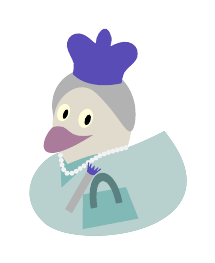
\begin{tikzpicture}
	\duck[
		body=qskin,
		bill=qbill,
		jacket=qdress,
		tshirt=teal!30!qdress,
		shorthair=gray!60!white,
		necklace=gray!10!white,
		handbag=teal!30!qdress
	]  
	\fill[gray!60!white,rotate=-30] (0.27,1.23) rectangle (0.37,0.65);
	\fill[qcrown,scale=0.23,rotate=-20,yshift=82,xshift=38] \duckpathqueencrown;
	\fill[qcrown,yshift=3] \duckpathkingcrown;
\end{tikzpicture}
	
\end{document}